\chapter{Elvégzett munka}


\section{Koncepció}
Állapottérképek formális verifikációjának támogatása MagicDraw-ban, egy plug-in fejlesztésével lett megvalósítva. A plug-in függ a Viatra For MagicDraw-tól, ami lehetővé teszi modellek transzformációját Viatra segítségével aminek a 2.0.1-es verziója van használva. A plug-in legfontosabb funkciója MagicDraw modellek Gamma modellekké való transzformációja. A letranszformált már Gamma nyelvű modelleket az keretrendszer kezelni tudja, a verifikáció elvégzéséhez az eszköznek csak egyes részei szükségesek (\ref{fig:used-gamma} ábra). A plug-in MagicDrawToGammának lett elnevezve.

\begin{figure}[!ht]
	\centering
	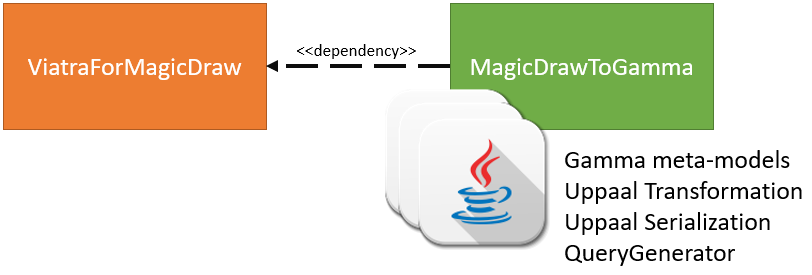
\includegraphics[keepaspectratio, width=120mm]{figures/plan.png}
	\caption{Architektúra koncepció}
	\label{fig:used-gamma}
\end{figure}

\section{Fejlesztőkörnyezet}
 A fejlesztés megkezdéséhez szükséges volt összeállítani egy olyan fejlesztőkörnyezetet amivel hatékonyan lehet plug-int fejleszteni. MagicDraw biztosít egy ún. skeletont Eclipsehez és IntelliJhez is plug-in fejlesztéséhez, de a fejlesztés nem ezek segítségével hanem az IncQueryLabs által készített skeleton felhasználásával valósult meg. Ez már elő volt készítve V4MD használatához.
 
A skeleton egy Eclipse project, viszont Gradlet használ a projekt fordításához és a dependenciák kezeléséhez, ez sokszor inkonzisztenciákhoz vezetett, az egyik legnagyobb probléma a Viatra Querik generálása amit Gradleel nem csak Eclipsel lehet generálni. A kódbázis egy része nem Javában hanem Xtendben íródott, a Viatra modell transzformációk implementálása ezzel a nyelvvel egyszerűbb, azok az osztályok melyeknél nem volt indokolt, jellemzően a MagicDraw felhasználói felületeinél, azok Java 8-ban lettek implementálva.

A dolgozat elkészítése idején a MagicDraw 19-es verziója is elérhető volt a plug-in azonban még nem ehhez, hanem a 18.5-ös verziójához készült. A kódbázis azonban kompatibilis lehet még az újabb verziókkal is, amennyiben az állapottérképeket érintő meta-modellek nem változnak.

Az eredeti koncepció  a Gamma implementációján nem kívánt változtatni, csak felhasználni azt, viszont a jelenlegi verziója Viatra 1.6 függőséggel rendelkezik ami problémákat okozott: a plug-in más verzióját használja a Viatranak , ezért az érintett Gamma függőségekben, az implementáció módosítva lett, hogy azok is Viatra 2-es Api-t használjanak.

Gamma a verifikációt Uppaal segítségével végzi el, ehhez előállít egy leírást a rendszerről és egy queryt ami a rendszerrel szemben támasztott követelményeket írja le. Utóbbi megírásához biztosít egy UI elemet amivel a felhasználó az Uppaal ismerete nélkül is képes a követelmények definiálására. Ez a funkció teljesen át lett emelve Gammából módosított implementációval a MagicDrawToGammába. A Gamma az Uppaalra az operációs rendszeren keresztül hív át, ezért az Uppaalt külön kell telepíteni és konfigurálni.

\subsection{MagicDraw - Gamma transzformáció}
